\documentclass[11pt]{article}

\usepackage[margin=1in]{geometry}
\usepackage{amsmath, amssymb}
\usepackage{booktabs}
\usepackage{enumitem}
\usepackage{hyperref}
\usepackage{setspace}
\usepackage{graphicx}
\usepackage{xcolor}
\usepackage{float}
\usepackage{caption}

\setstretch{1.15}
\graphicspath{{figures/}}

% --------------------
% Course info
% --------------------
\newcommand{\course}{ST5230: Applied Natural Language Processing}
\newcommand{\semester}{Semester 2, AY2025/2026}

\title{\textbf{Do LLM Rankings Change if You Ask Differently?}\\
\large Evaluating Ranking Reversals under Non-semantic Prompt Perturbations and Subset Resampling}
\author{Group 14\\
ZHANG QIANCHI, PENG YANGYUNZHI, JIANG YIFAN, MENG XIANGCHEN}
\date{}

\begin{document}
\maketitle
\vspace{-1em}

\begin{abstract}
Large language model leaderboards usually present benchmark performance as a single ordered list, implicitly assuming that the ordering is stable under reasonable evaluation choices. This project tests that assumption by studying whether non-semantic prompt perturbations and evaluation-subset variation can change model rankings. We evaluate four models, GPT-4o-mini, Gemini-2.0-flash, Qwen-2.5-7B, and Llama-3.1-8B, on MMLU, ARC-Challenge, and HellaSwag. The main dataset-level experiment uses 900 questions, four task-preserving prompt templates, and 14,400 model responses. We then compute accuracy, prompt-wise ranking reversal rate (PRRR), subset ranking reversal rate (SRRR), and rank-probability summaries using 1,000 half-subset resampling iterations per scope. We further run an expanded MMLU subject-level analysis over five subjects with 200 questions per subject. The central finding is that ranking stability is highly task-dependent: ARC-Challenge is comparatively robust, MMLU has a stable top model but less stable lower ranks, and HellaSwag is substantially more fragile. At the subject level, MMLU instability can be even stronger, with high-school world history reaching a maximum PRRR of 74.30\% and sociology reaching a maximum SRRR of 67.90\%. These results show that leaderboard interpretation should distinguish average accuracy from ranking robustness.
\end{abstract}

\section{Introduction}

Leaderboards are a convenient interface for large language model (LLM) evaluation. A model receives a benchmark score, models are sorted by that score, and the resulting order is often interpreted as a stable statement about relative capability. This convention is useful, but it hides a strong assumption: if the evaluation protocol is changed in a reasonable but non-semantic way, the ranking should remain mostly unchanged.

That assumption is not guaranteed. Even when the underlying task is fixed, prompt wording, instruction style, and answer formatting can affect model behavior. Similarly, the observed ranking may depend on which subset of examples is evaluated. If the gap between two models is small, prompt variation or subset noise can be large enough to change the apparent winner.

This project studies LLM evaluation through the lens of \textbf{ranking stability}. Instead of asking only which model has the highest average accuracy, we ask whether that ordering survives prompt perturbations and subset resampling. This framing matters because downstream users often care about rank comparisons: which model is best, which model is second, and whether a reported improvement is robust or only a point-estimate artifact.

Our contributions are:
\begin{itemize}[leftmargin=*]
    \item We construct a controlled benchmark experiment with four task-preserving prompt templates across MMLU, ARC-Challenge, and HellaSwag.
    \item We separate two sources of instability: prompt-induced ranking changes and subset-induced ranking changes.
    \item We report PRRR and SRRR as ranking stability diagnostics, showing that HellaSwag is much less stable than ARC-Challenge and MMLU at the dataset level.
    \item We extend the analysis to expanded MMLU subject subsets and show that subdomain-level ranking instability can be much larger than aggregate benchmark-level instability.
\end{itemize}

\section{Related Work}

This work connects to three lines of prior research. First, benchmark construction work such as MMLU, ARC, and HellaSwag defines widely used multiple-choice evaluation settings for knowledge, reasoning, and commonsense completion tasks \cite{hendrycks2020mmlu, clark2018arc, zellers2019hellaswag}. These benchmarks provide convenient automatically scorable testbeds, but benchmark papers do not necessarily establish that model rankings are invariant to prompt and subset variation.

Second, prompt robustness work shows that LLM outputs can be sensitive to prompt form even when the task semantics remain unchanged. PromptRobust, for example, studies robustness under adversarial prompt perturbations and demonstrates that prompt design can materially affect downstream performance \cite{zhu2023promptrobust}. Our work differs by focusing on whether such variation changes the \emph{ordering} between models, not only their individual scores.

Third, recent evaluation reliability discussions emphasize uncertainty, repeated trials, and error bars in LLM evaluation \cite{miller2024errorbars, fourrier2024openllm}. We build on this perspective by treating a leaderboard as an empirical object whose robustness should be measured. Our project is therefore closer to a stress test for leaderboard interpretation than a search for the best-performing model.

\section{Experimental Setup}

\subsection{Research Question}

We study the following testable question:
\begin{quote}
Does model ranking remain stable under task-preserving prompt perturbations and evaluation-subset variation?
\end{quote}

We operationalize this question using two types of ranking reversal. Prompt-wise ranking reversal measures whether two prompt templates induce different rankings on the same resampled item subset. Subset ranking reversal measures whether a resampled subset induces a different ranking from the full item set under the same prompt.

\subsection{Models}

We evaluate four models through the OpenRouter API:
\begin{itemize}[leftmargin=*]
    \item \texttt{openai/gpt-4o-mini} (GPT-4o-mini)
    \item \texttt{google/gemini-2.0-flash-001} (Gemini-2.0-flash)
    \item \texttt{qwen/qwen-2.5-7b-instruct} (Qwen-2.5-7B)
    \item \texttt{meta-llama/llama-3.1-8b-instruct} (Llama-3.1-8B)
\end{itemize}

All model calls use temperature $0$ and \texttt{max\_tokens=150}. This deterministic decoding setting reduces sampling randomness so that the analysis focuses on prompt and item-subset variation.

\subsection{Datasets and Tasks}

\begin{center}
\begin{tabular}{@{}p{0.22\linewidth} p{0.18\linewidth} p{0.50\linewidth}@{}}
\toprule
\textbf{Dataset} & \textbf{Size} & \textbf{Details} \\
\midrule
MMLU & 300 & Main dataset-level sample; 50 questions from each of 6 subjects in the test split. \\
ARC-Challenge & 300 & Science question answering benchmark; sampled from the official test split. \\
HellaSwag & 300 & Commonsense sentence-completion benchmark; sampled from validation because test labels are not public. \\
Expanded MMLU subjects & 5 $\times$ 200 & Subject-level analysis over \texttt{conceptual\_physics}, \texttt{high\_school\_mathematics}, \texttt{philosophy}, \texttt{high\_school\_world\_history}, and \texttt{sociology}. \\
\bottomrule
\end{tabular}
\end{center}

\subsection{Prompt Design}

Each question is converted into four prompt templates that preserve the answer options and task semantics while varying surface form:
\begin{itemize}[leftmargin=*]
    \item \textbf{T1 Minimal}: the question and choices followed by ``Select one option.''
    \item \textbf{T2 Benchmark}: explicit multiple-choice framing, with ``Question'' and ``Options'' fields.
    \item \textbf{T3 Natural}: conversational framing, e.g., ``I have a multiple-choice question for you.''
    \item \textbf{T4 Order/Phrasing}: same task and options, but with altered instruction order and phrasing.
\end{itemize}

The main dataset-level experiment therefore expands 900 items into $900 \times 4 = 3600$ prompt requests. Running four models over these requests yields $3600 \times 4 = 14400$ model responses. The expanded MMLU subject experiment adds 1000 subject-level questions, 4000 prompt requests, and 16000 responses.

\subsection{Scoring}

All tasks are multiple-choice. We parse each model output into one of \texttt{A/B/C/D} and compare it with the gold label to obtain a binary score. In the main dataset-level experiment, there are 3 parse failures out of 14,400 responses. In the expanded MMLU subject experiment, there are no parse failures.

\section{Metrics and Statistical Protocol}

\subsection{Accuracy and Ranking}

For an item set $P$, prompt template $T$, and model $m$, let
\[
\mathrm{Acc}(P,T,m)
=
\frac{1}{|P|}\sum_{x\in P} s(x,T,m),
\]
where $s(x,T,m)\in\{0,1\}$ is the fixed binary correctness score for model $m$ on item $x$ under template $T$. The ranking $R_{P,T}$ is the ordering of the four models by $\mathrm{Acc}(P,T,m)$.

\subsection{Prompt-wise Ranking Reversal Rate}

Prompt-wise Ranking Reversal Rate (PRRR) captures whether two prompt templates induce different rankings on the same resampled subset. For an item set $P$, baseline template $T_1$, comparison template $T_2$, and resampled subsets $P_i\subset P$ for $i=1,\ldots,N$,
\[
\mathrm{PRRR}(P,T_1,T_2)
=
\frac{1}{N}
\sum_{i=1}^{N}
\mathbf{1}\left[R_{P_i,T_1}\neq R_{P_i,T_2}\right].
\]
In this project, $T_1$ is the minimal instruction template and $T_2$ ranges over the three non-minimal templates.

\subsection{Subset Ranking Reversal Rate}

Subset Ranking Reversal Rate (SRRR) captures whether a subset ranking differs from the full-set ranking under the same prompt template:
\[
\mathrm{SRRR}(P,T)
=
\frac{1}{N}
\sum_{i=1}^{N}
\mathbf{1}\left[R_{P,T}\neq R_{P_i,T}\right].
\]
PRRR isolates prompt-to-prompt disagreement, while SRRR isolates instability caused by using an incomplete evaluation subset.

\subsection{Resampling Protocol}

For each dataset or subject scope, we run $N=1000$ resampling iterations. Each iteration samples a half-sized subset without replacement from the current scope. For the main 300-item datasets, each subset contains 150 items. For each expanded MMLU subject, each subset contains 100 of the 200 subject items.

\section{Results}

\subsection{Dataset-level Accuracy}

Table~\ref{tab:acc} reports prompt-averaged accuracy and rank for the main dataset-level experiment. Gemini is first on ARC-Challenge and MMLU, while GPT-4o-mini is first on HellaSwag.

\begin{table}[H]
\centering
\caption{Prompt-averaged dataset-level accuracy.}
\label{tab:acc}
\begin{tabular}{@{}llcc@{}}
\toprule
\textbf{Dataset} & \textbf{Model} & \textbf{Accuracy} & \textbf{Rank} \\
\midrule
ARC-Challenge & Gemini-2.0-flash & 94.00\% & 1 \\
ARC-Challenge & GPT-4o-mini & 90.83\% & 2 \\
ARC-Challenge & Qwen-2.5-7B & 85.08\% & 3 \\
ARC-Challenge & Llama-3.1-8B & 77.33\% & 4 \\
\midrule
HellaSwag & GPT-4o-mini & 89.17\% & 1 \\
HellaSwag & Gemini-2.0-flash & 87.25\% & 2 \\
HellaSwag & Qwen-2.5-7B & 84.25\% & 3 \\
HellaSwag & Llama-3.1-8B & 68.33\% & 4 \\
\midrule
MMLU & Gemini-2.0-flash & 85.08\% & 1 \\
MMLU & GPT-4o-mini & 73.42\% & 2 \\
MMLU & Qwen-2.5-7B & 70.33\% & 3 \\
MMLU & Llama-3.1-8B & 60.08\% & 4 \\
\bottomrule
\end{tabular}
\end{table}

\begin{figure}[H]
\centering
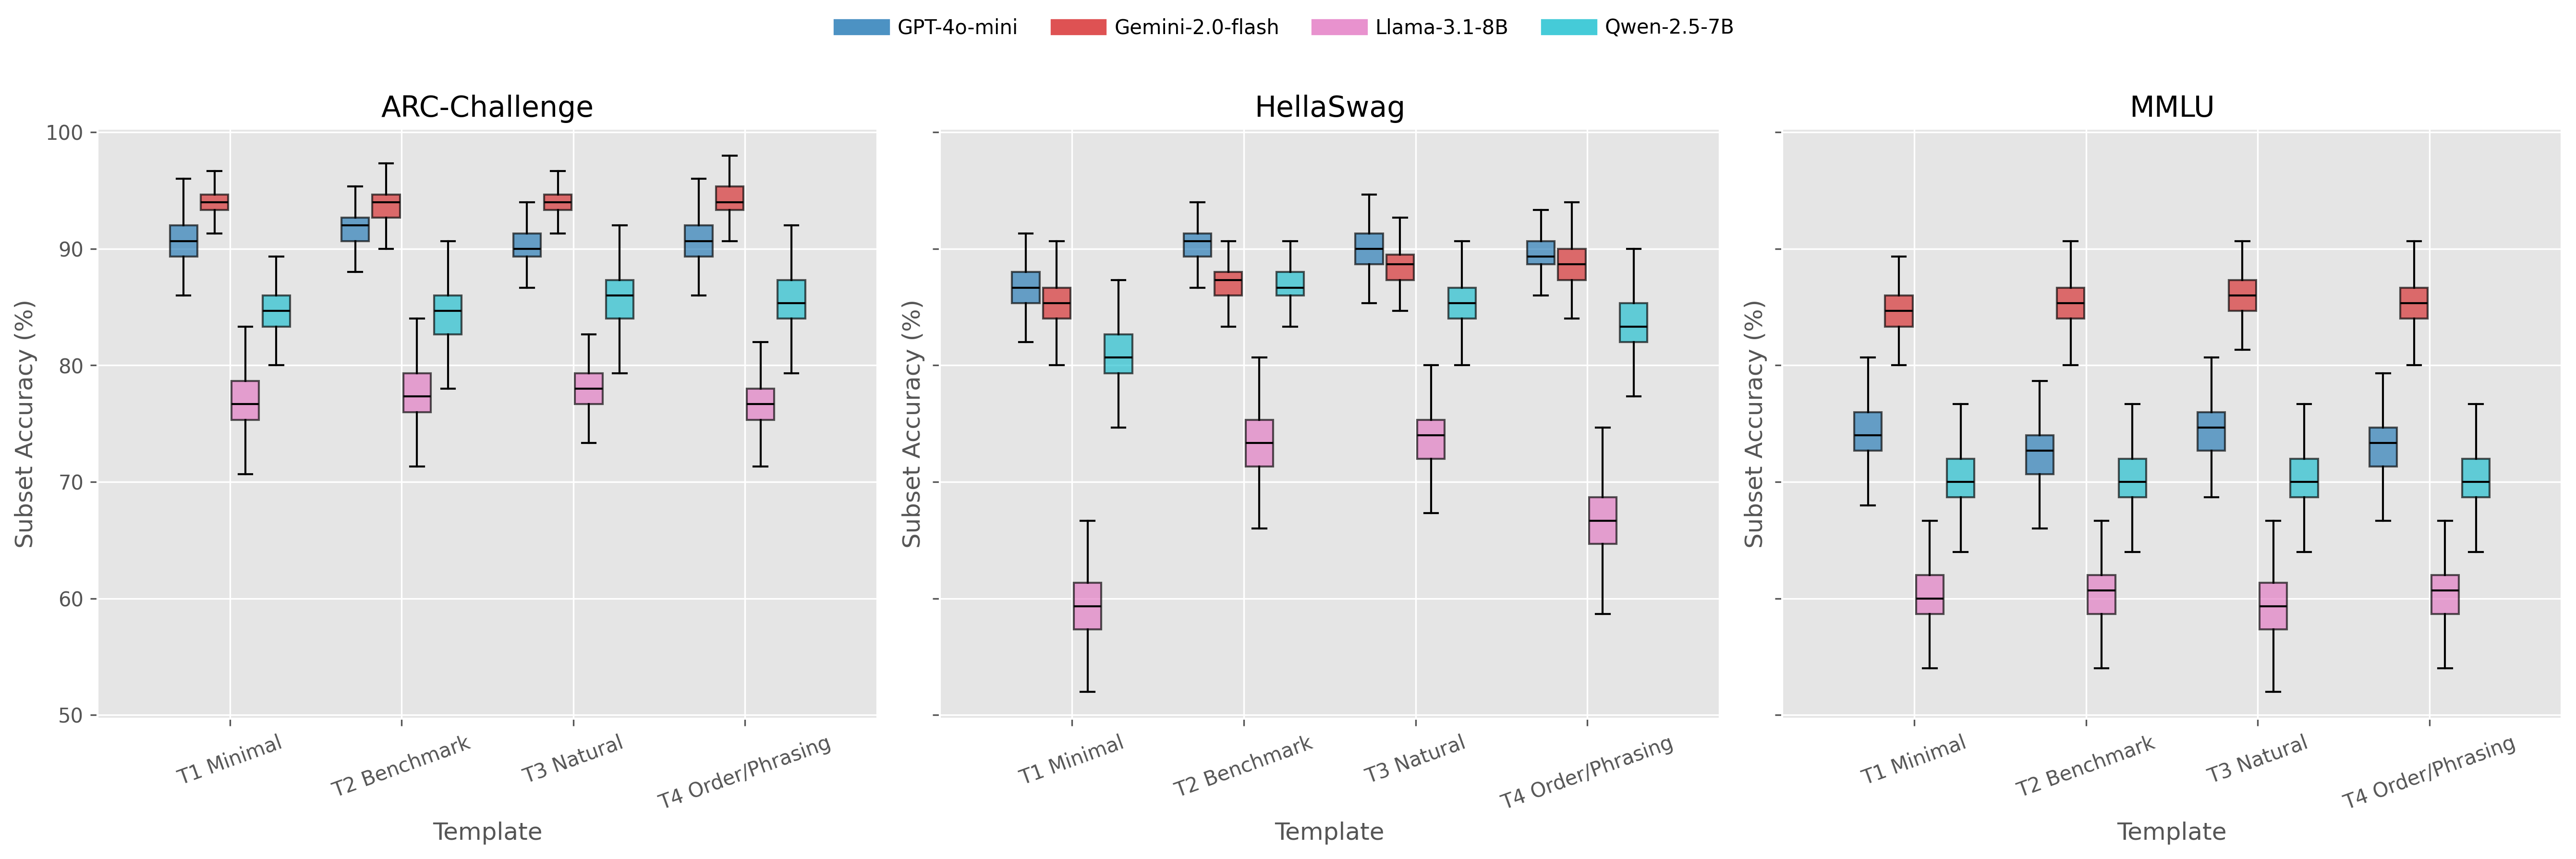
\includegraphics[width=\linewidth]{accuracy_boxplots.png}
\caption{Subset accuracy distributions across datasets, models, and prompt templates. ARC-Challenge has relatively separated model distributions, while HellaSwag and parts of MMLU show closer margins.}
\label{fig:accuracy}
\end{figure}

\subsection{Dataset-level Ranking Reversal}

Table~\ref{tab:dataset_rrr} summarizes the maximum PRRR and maximum SRRR observed for each benchmark. HellaSwag is the most fragile dataset in both prompt-induced and subset-induced ranking instability.

\begin{table}[H]
\centering
\caption{Maximum dataset-level PRRR and SRRR.}
\label{tab:dataset_rrr}
\begin{tabular}{@{}lcc@{}}
\toprule
\textbf{Dataset} & \textbf{Max PRRR} & \textbf{Max SRRR} \\
\midrule
ARC-Challenge & 10.60\% & 11.20\% \\
HellaSwag & 56.00\% & 42.80\% \\
MMLU & 15.60\% & 17.50\% \\
\bottomrule
\end{tabular}
\end{table}

\begin{figure}[H]
\centering
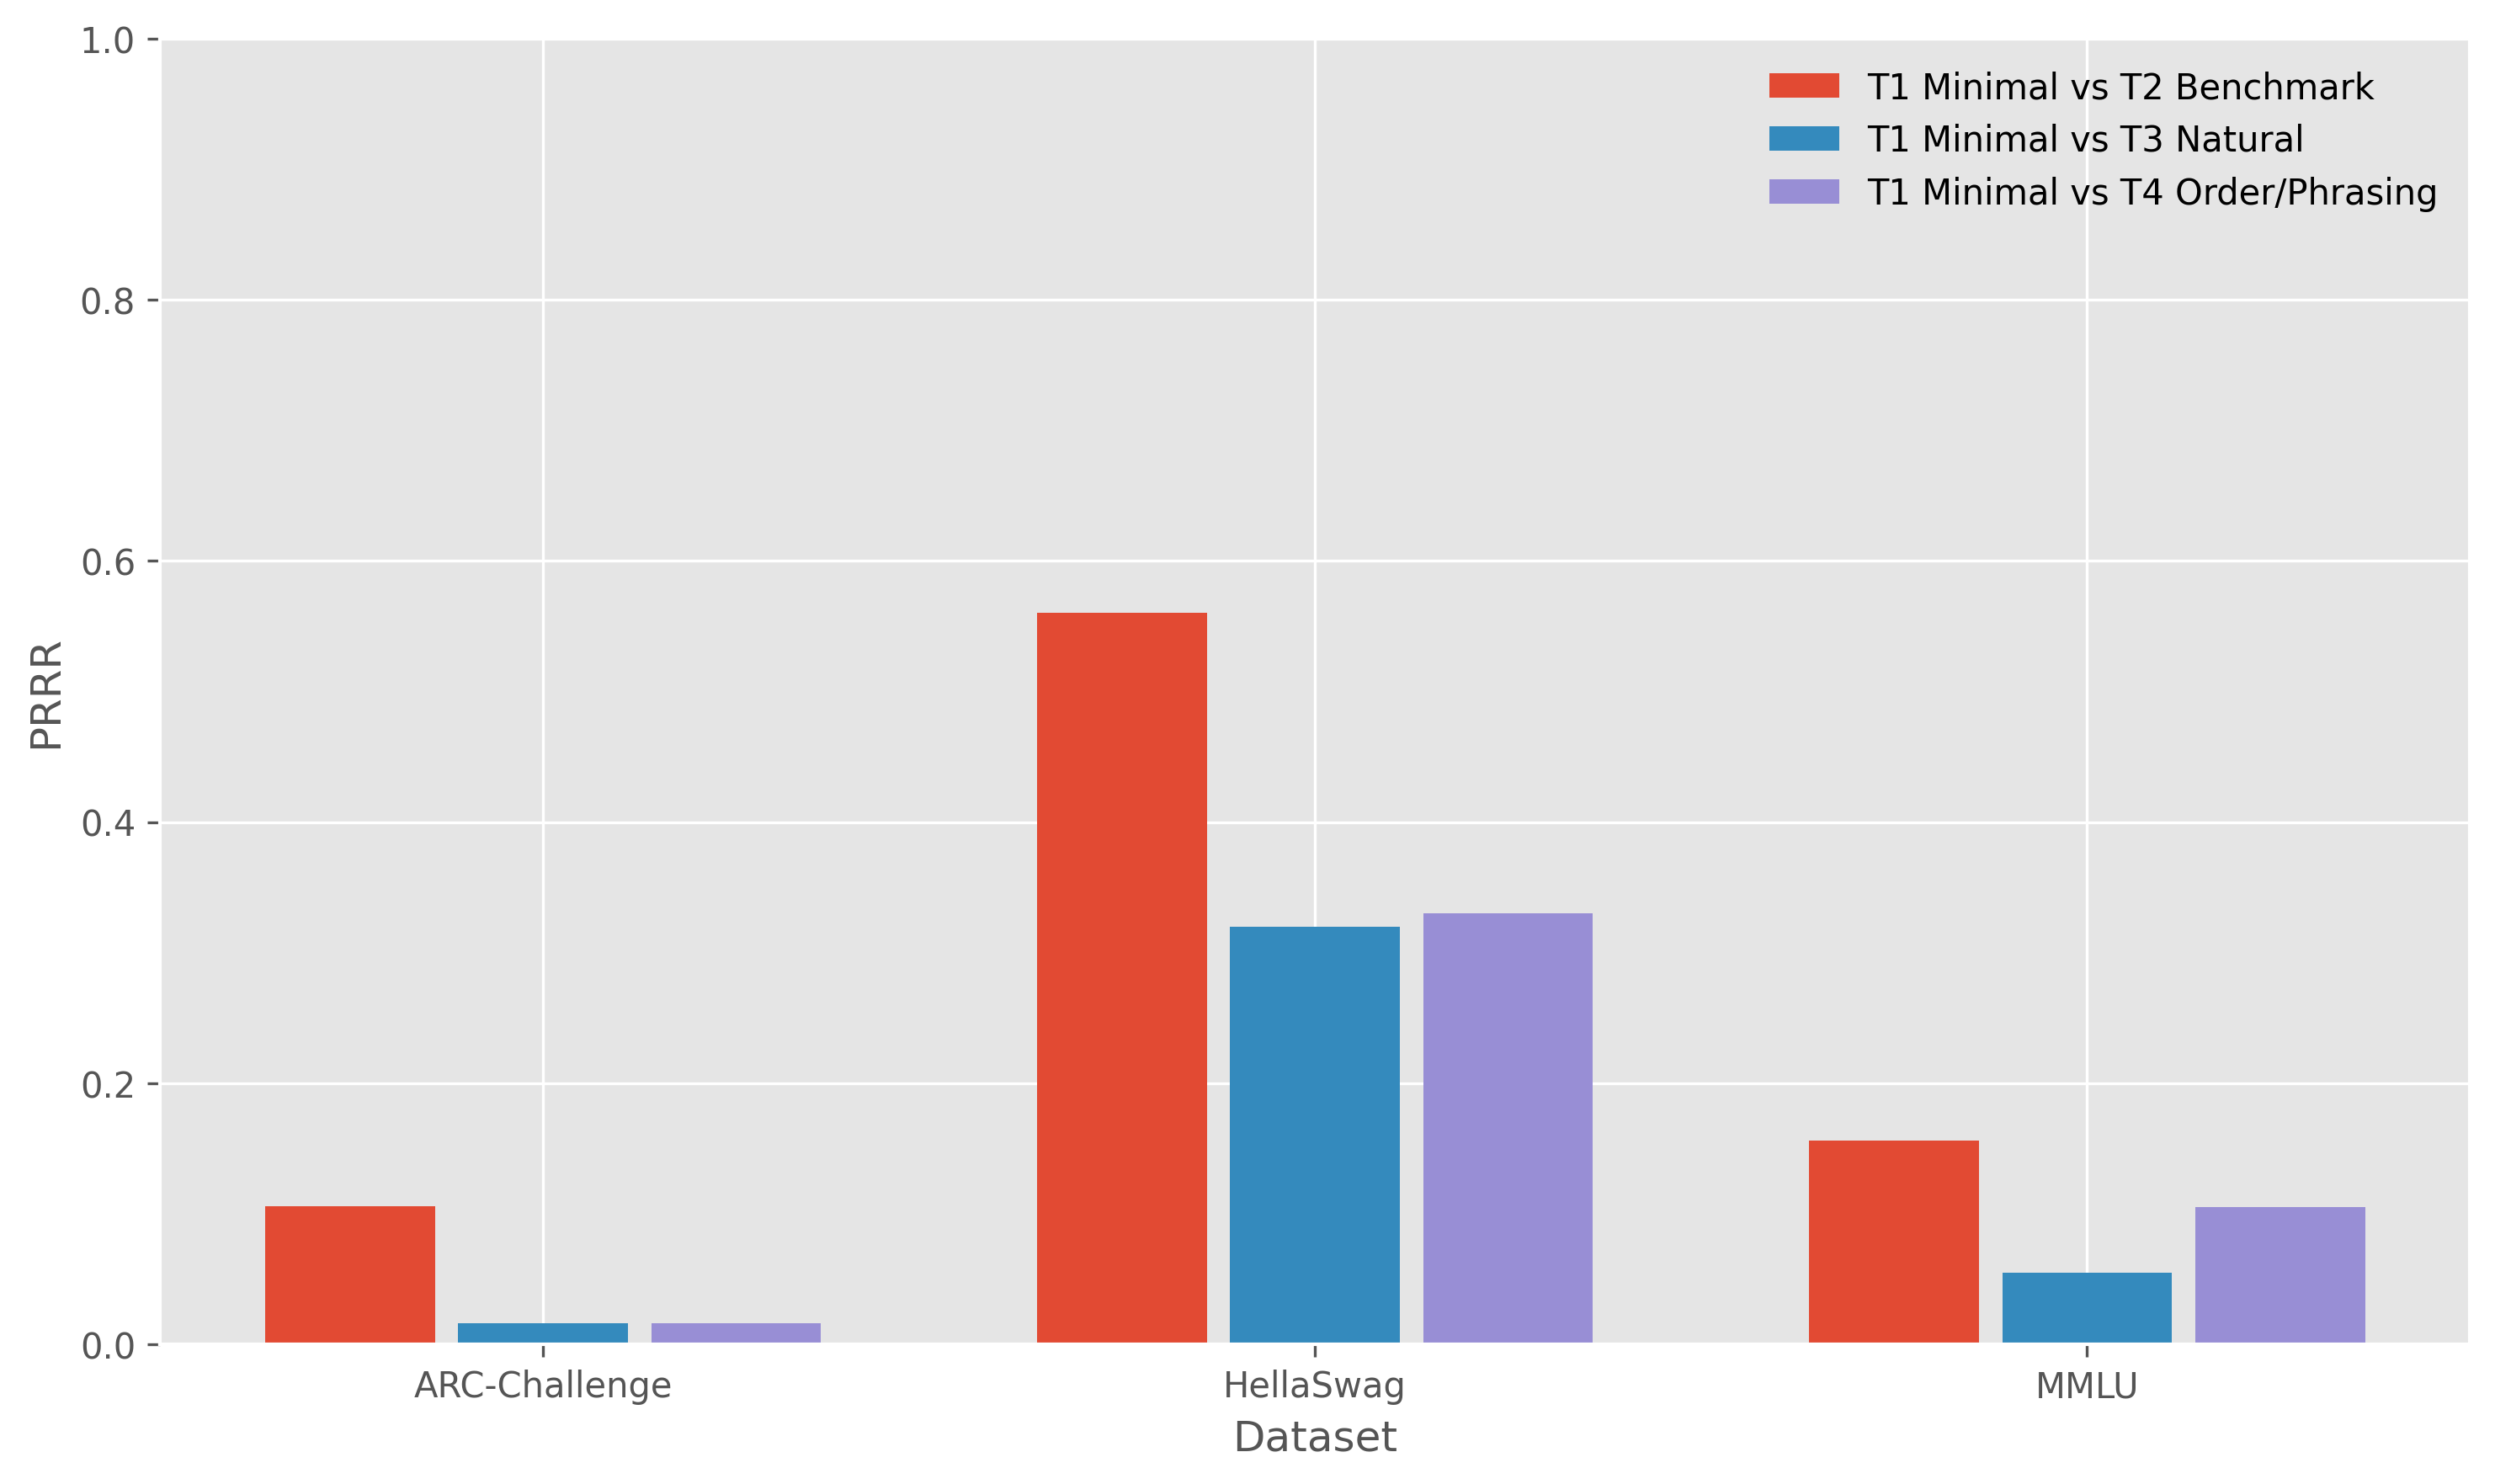
\includegraphics[width=0.82\linewidth]{prompt_ranking_reversal_rate.png}
\caption{Prompt-wise ranking reversal rate (PRRR). HellaSwag has the largest prompt-induced reversal rate, especially between the minimal and benchmark-style prompts.}
\label{fig:prrr}
\end{figure}

\begin{figure}[H]
\centering
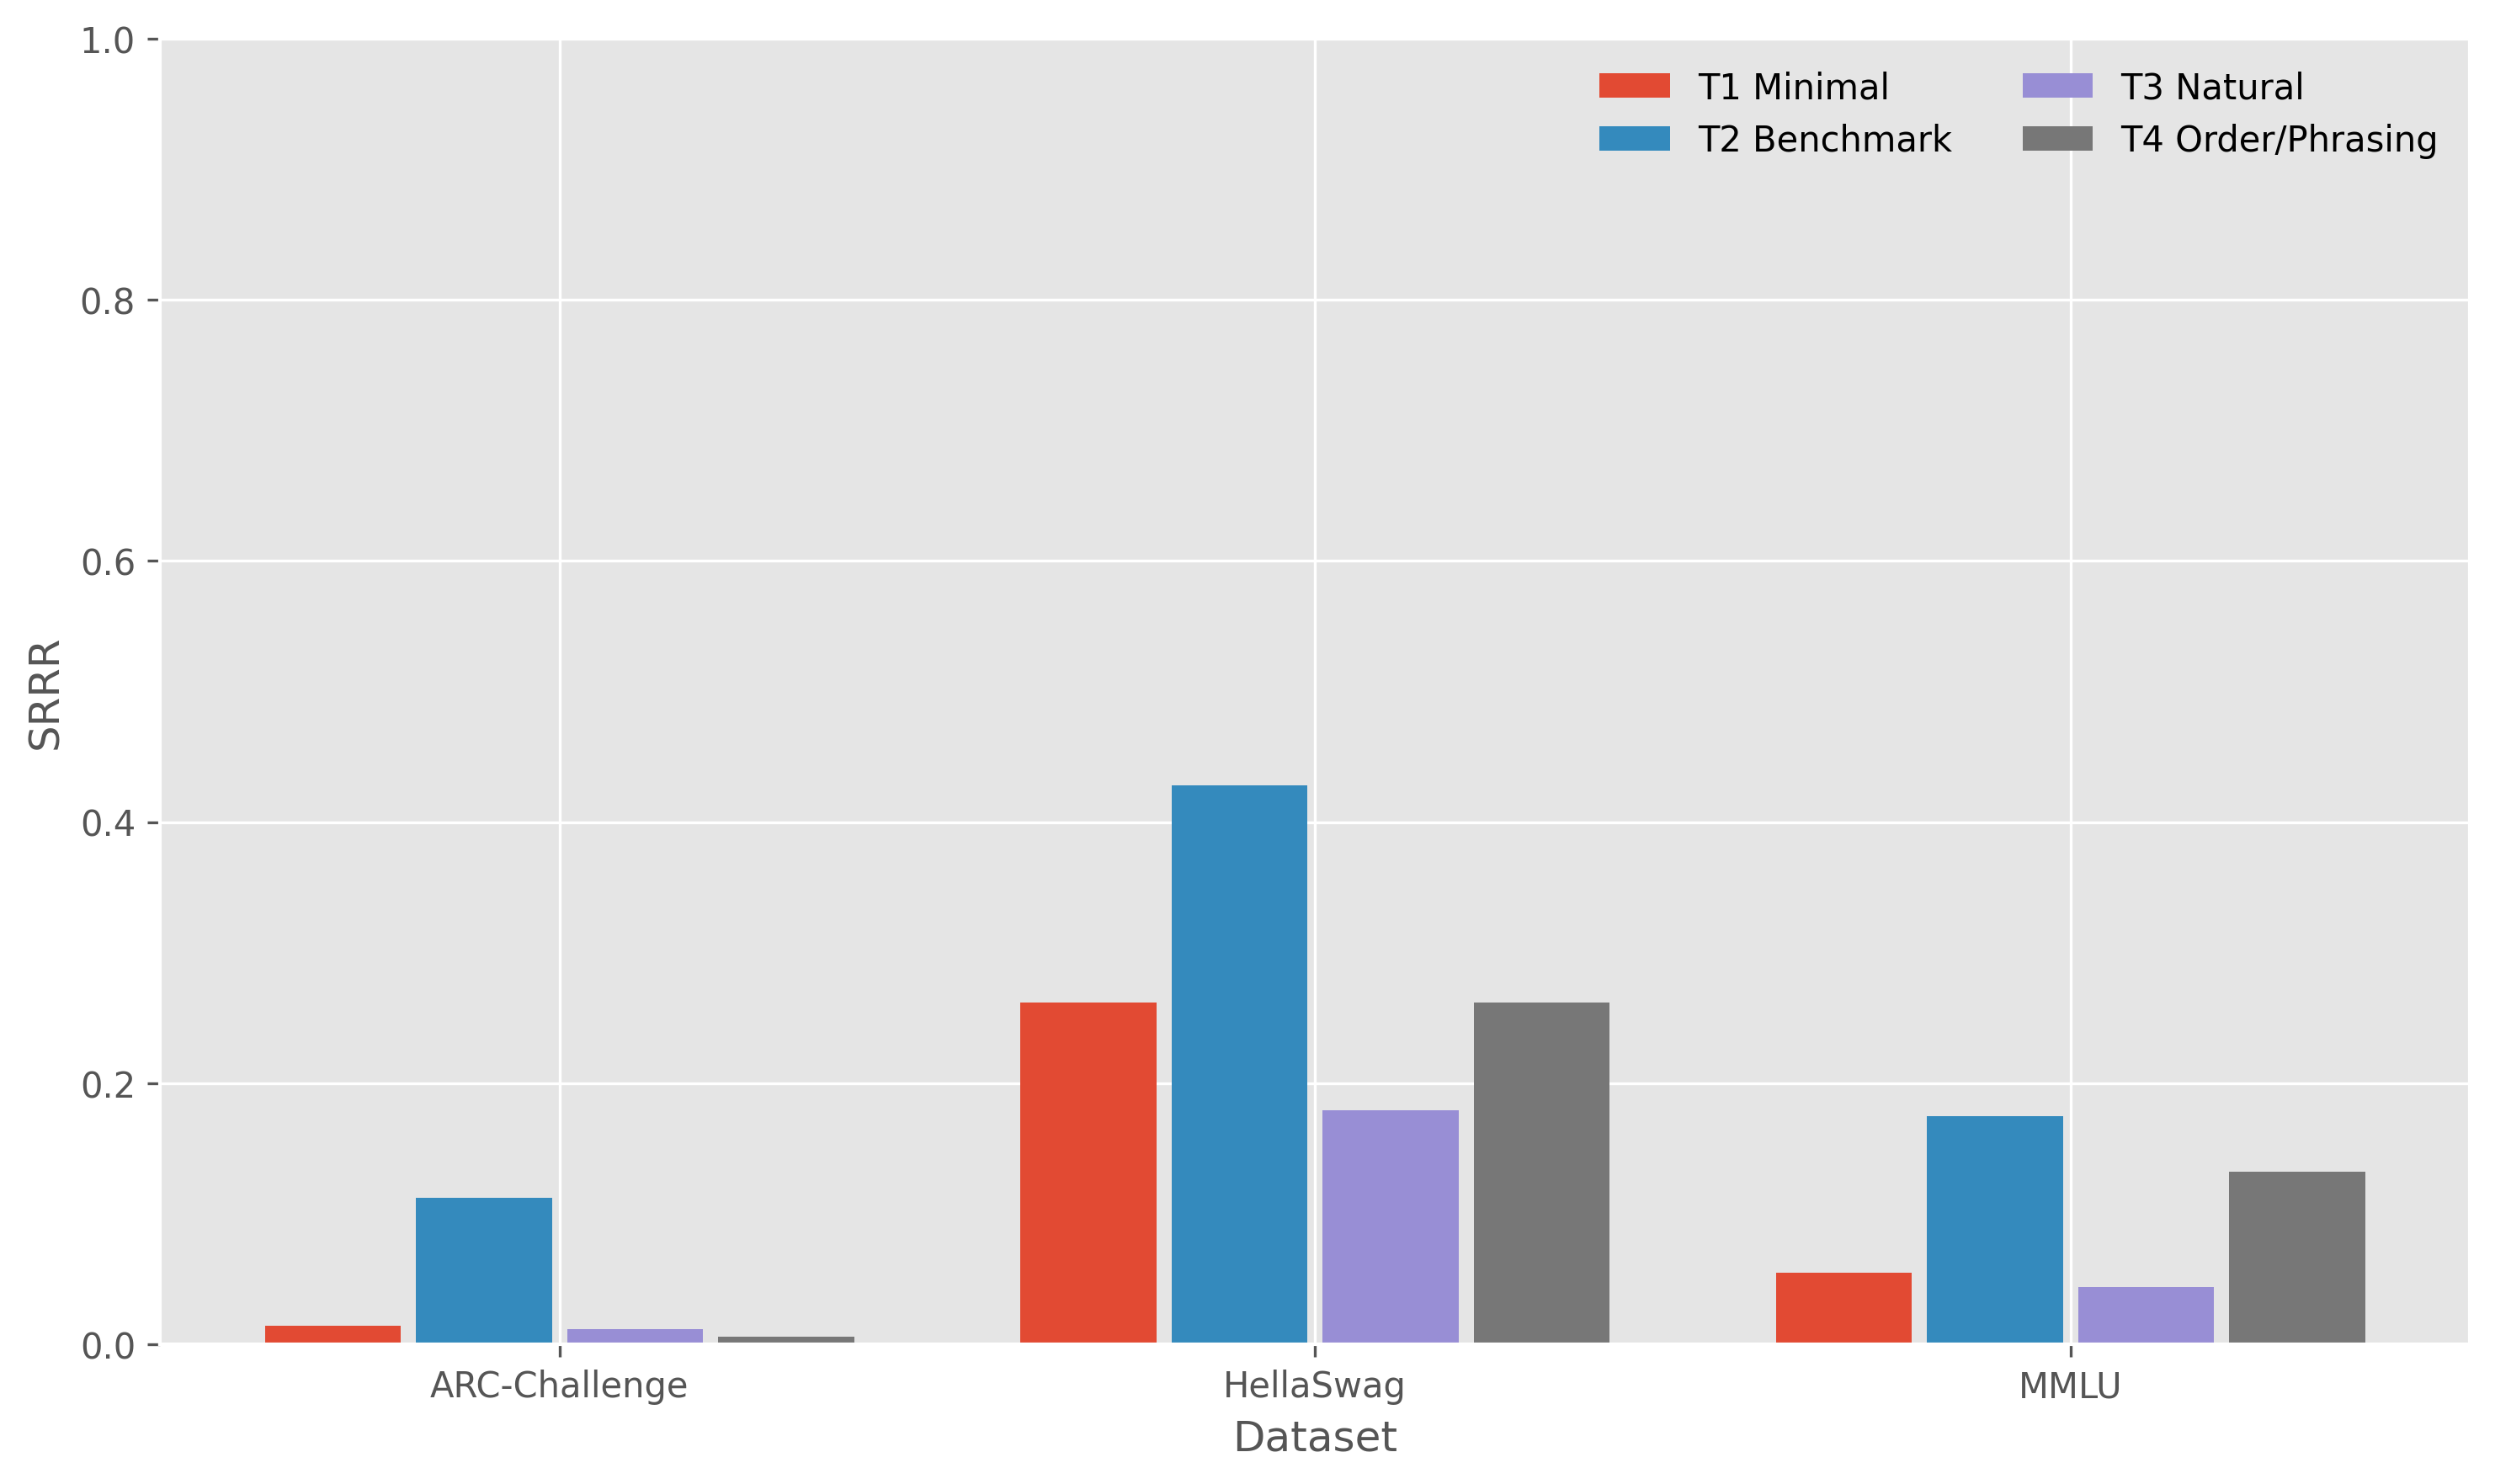
\includegraphics[width=0.82\linewidth]{subset_ranking_reversal_rate.png}
\caption{Subset ranking reversal rate (SRRR). HellaSwag is also most sensitive to using only a half-sized evaluation subset.}
\label{fig:srrr}
\end{figure}

\subsection{Expanded MMLU Subject-level Analysis}

The expanded MMLU subject experiment reveals substantially stronger instability than the aggregate MMLU result. Table~\ref{tab:mmlu_subject} reports the top model, top accuracy, maximum PRRR, and maximum SRRR for each subject.

\begin{table}[H]
\centering
\caption{Expanded MMLU subject-level stability results.}
\label{tab:mmlu_subject}
\begin{tabular}{@{}lccc@{}}
\toprule
\textbf{Subject} & \textbf{Winner} & \textbf{Max PRRR} & \textbf{Max SRRR} \\
\midrule
high\_school\_mathematics & Gemini-2.0-flash & 32.20\% & 38.70\% \\
conceptual\_physics & Gemini-2.0-flash & 25.60\% & 26.20\% \\
high\_school\_world\_history & Gemini-2.0-flash & 74.30\% & 55.00\% \\
philosophy & Gemini-2.0-flash & 56.10\% & 49.00\% \\
sociology & GPT-4o-mini & 54.30\% & 67.90\% \\
\bottomrule
\end{tabular}
\end{table}

\begin{figure}[H]
\centering
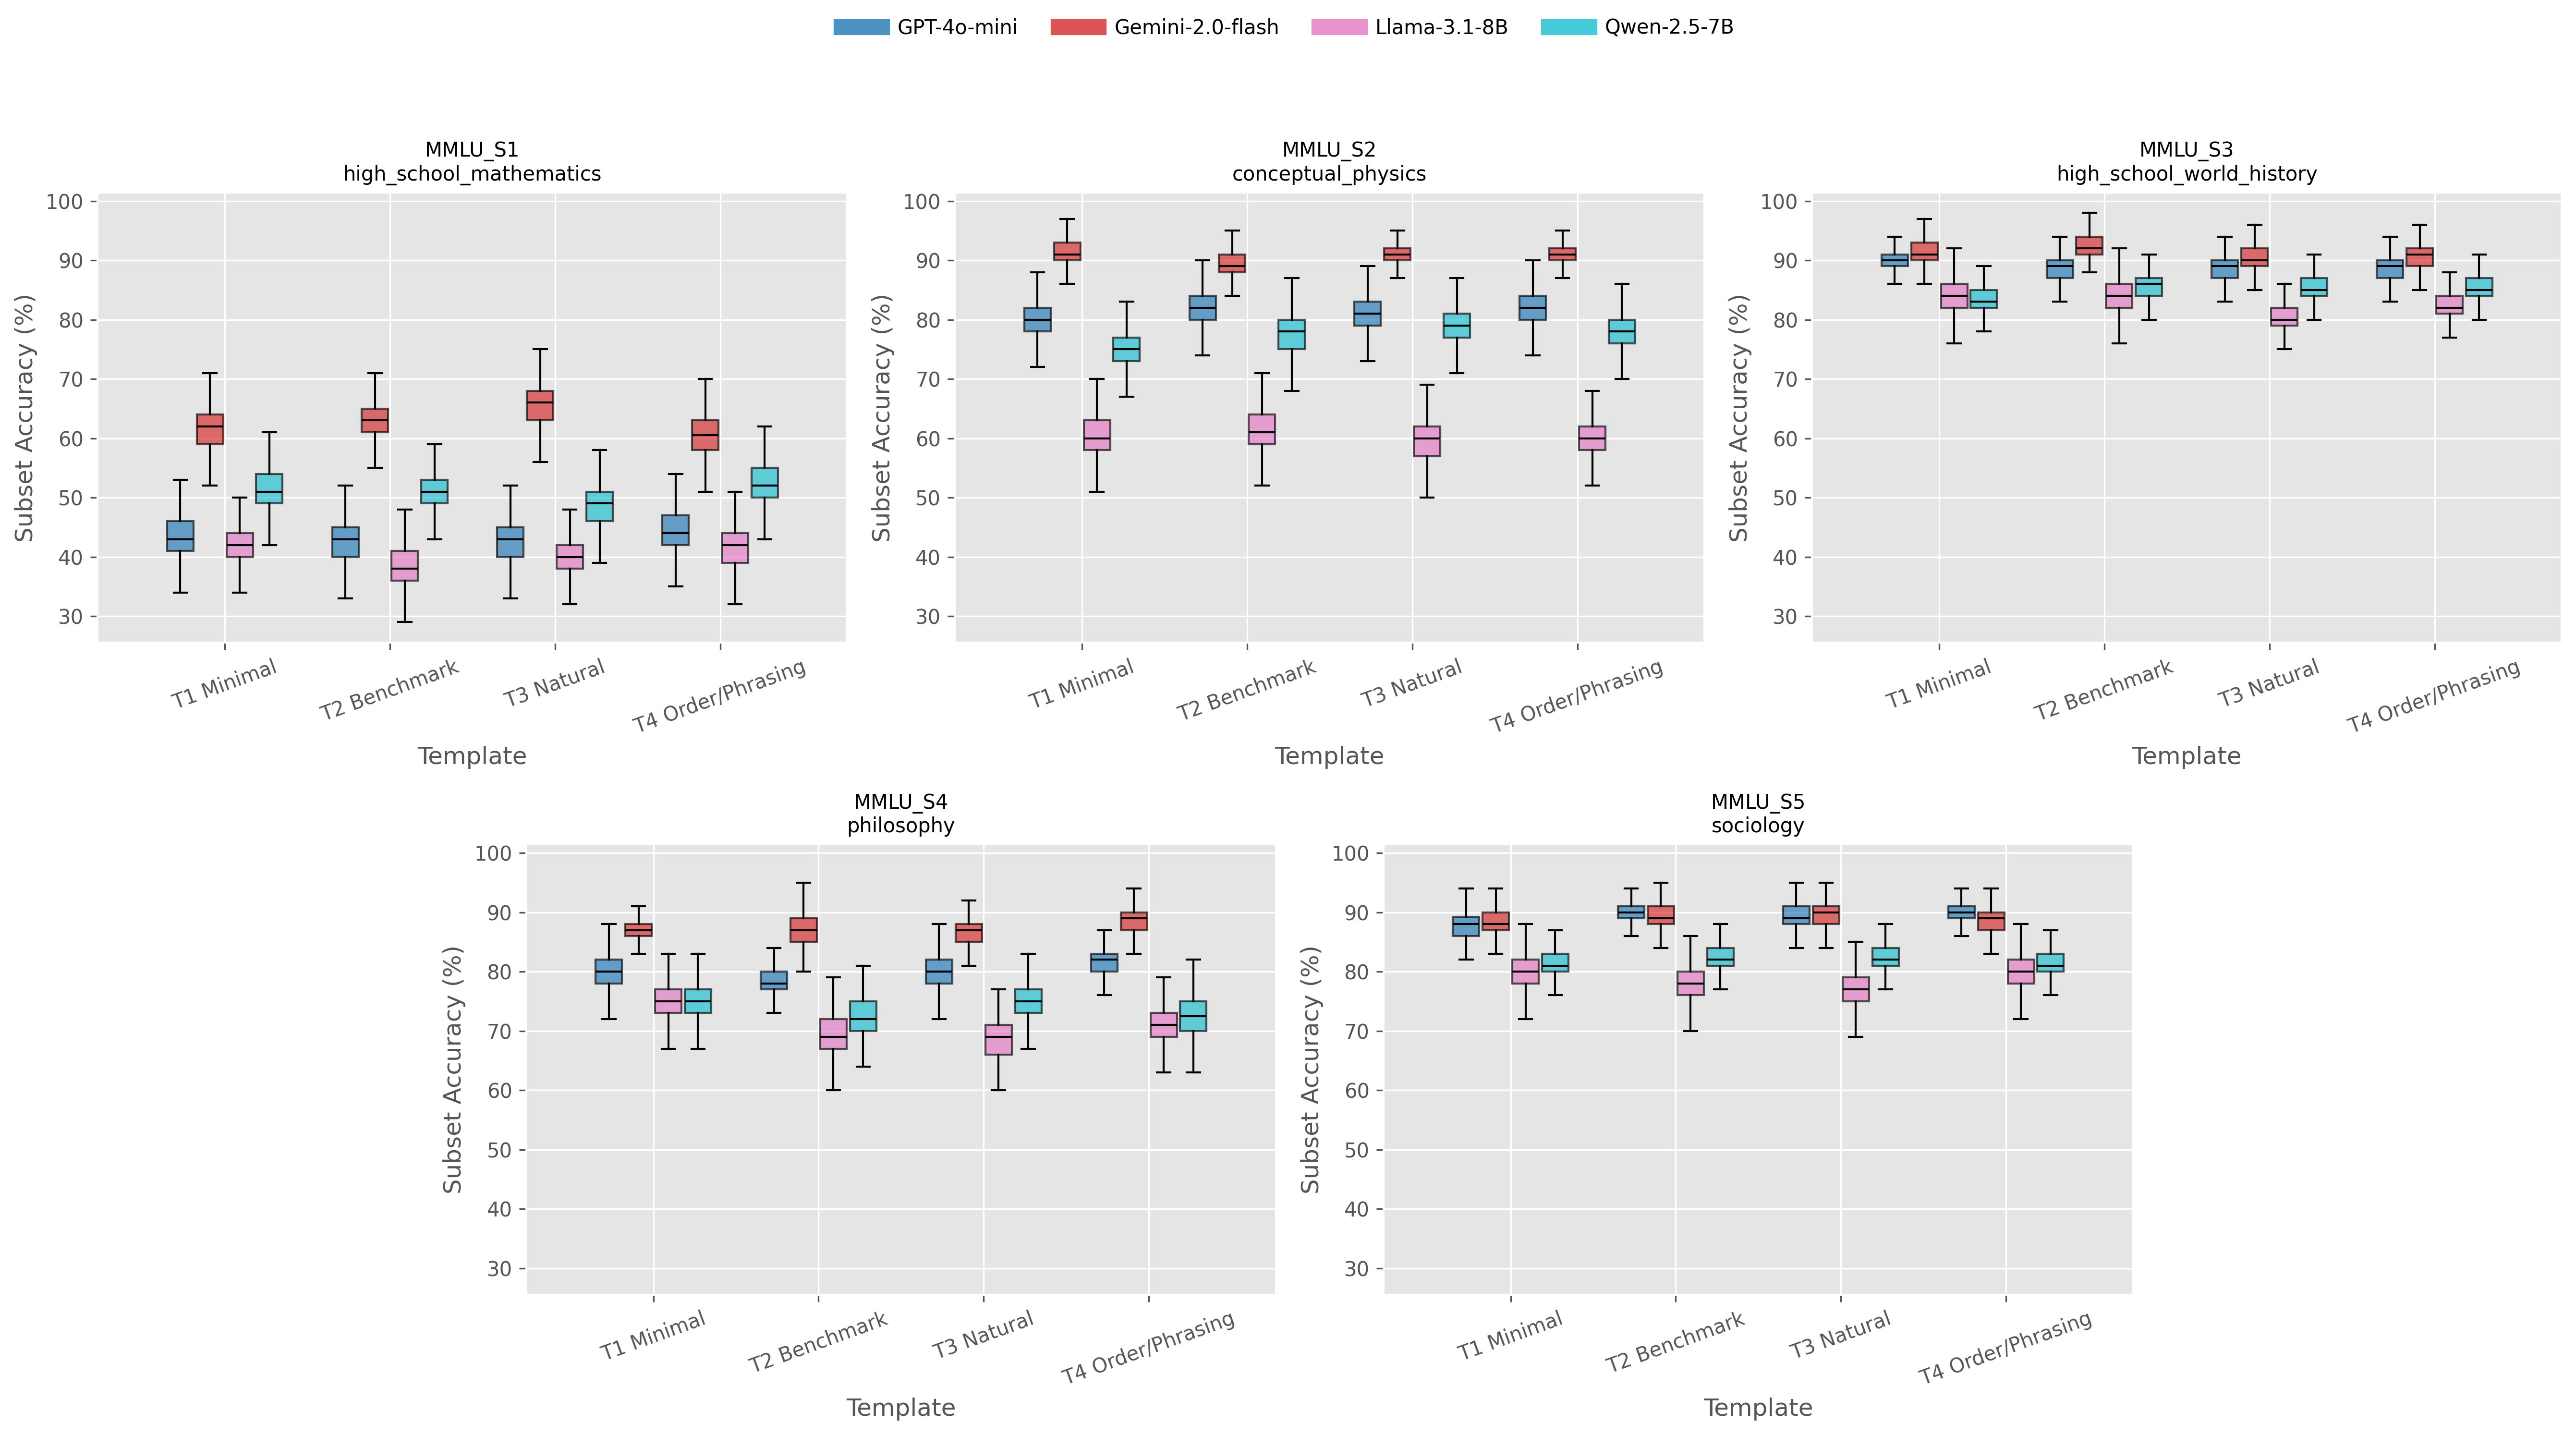
\includegraphics[width=\linewidth]{mmlu_subject_expanded_accuracy_boxplots.png}
\caption{Expanded MMLU subject-level subset accuracy distributions. The subject-level view exposes more heterogeneous margins than the aggregate benchmark view.}
\label{fig:mmlu_acc}
\end{figure}

\begin{figure}[H]
\centering
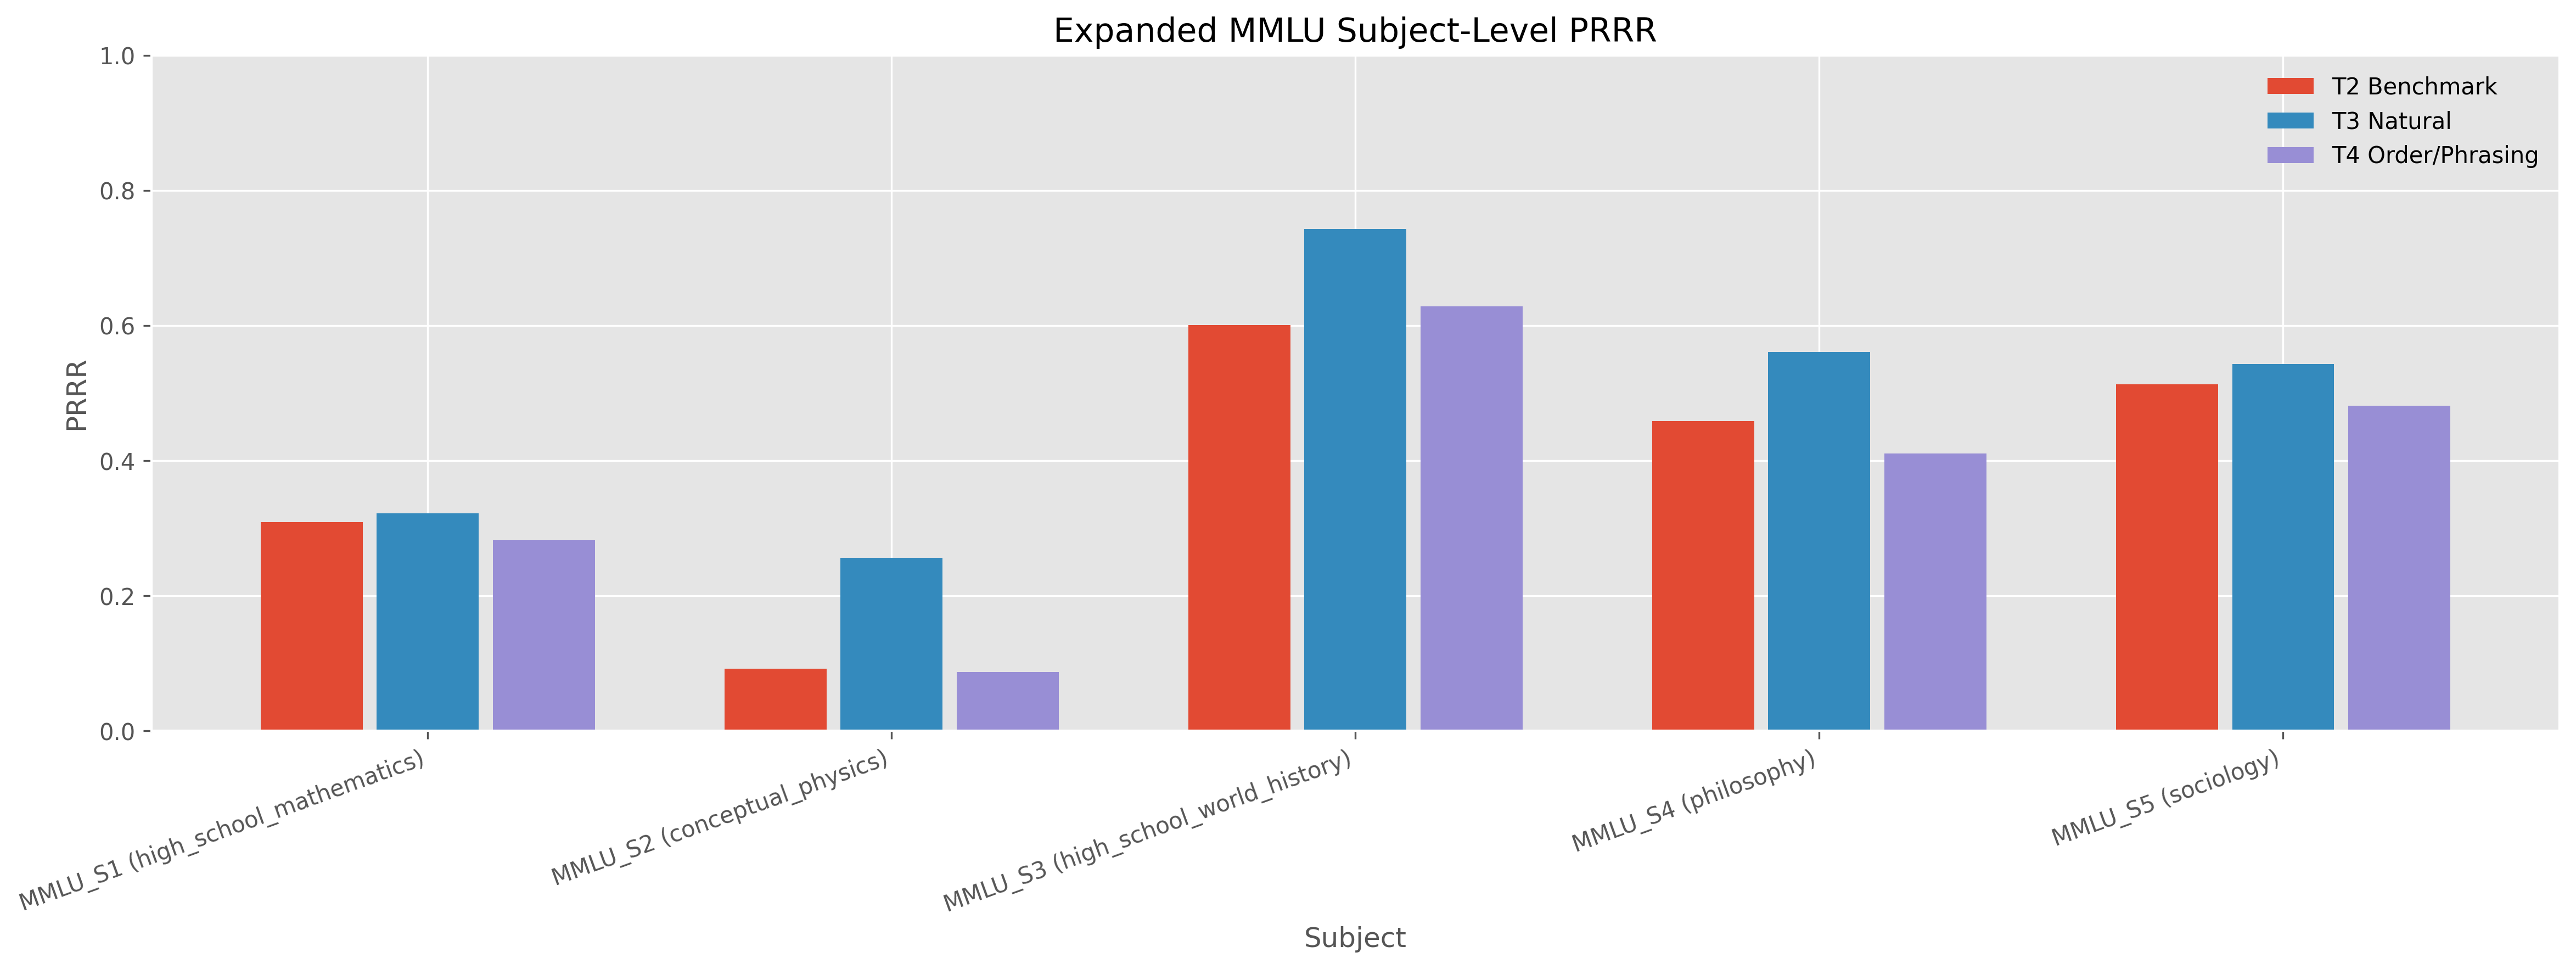
\includegraphics[width=\linewidth]{mmlu_subject_expanded_prrr.png}
\caption{Expanded MMLU subject-level PRRR. High-school world history and sociology exhibit particularly large prompt-induced ranking disagreement.}
\label{fig:mmlu_prrr}
\end{figure}

\begin{figure}[H]
\centering
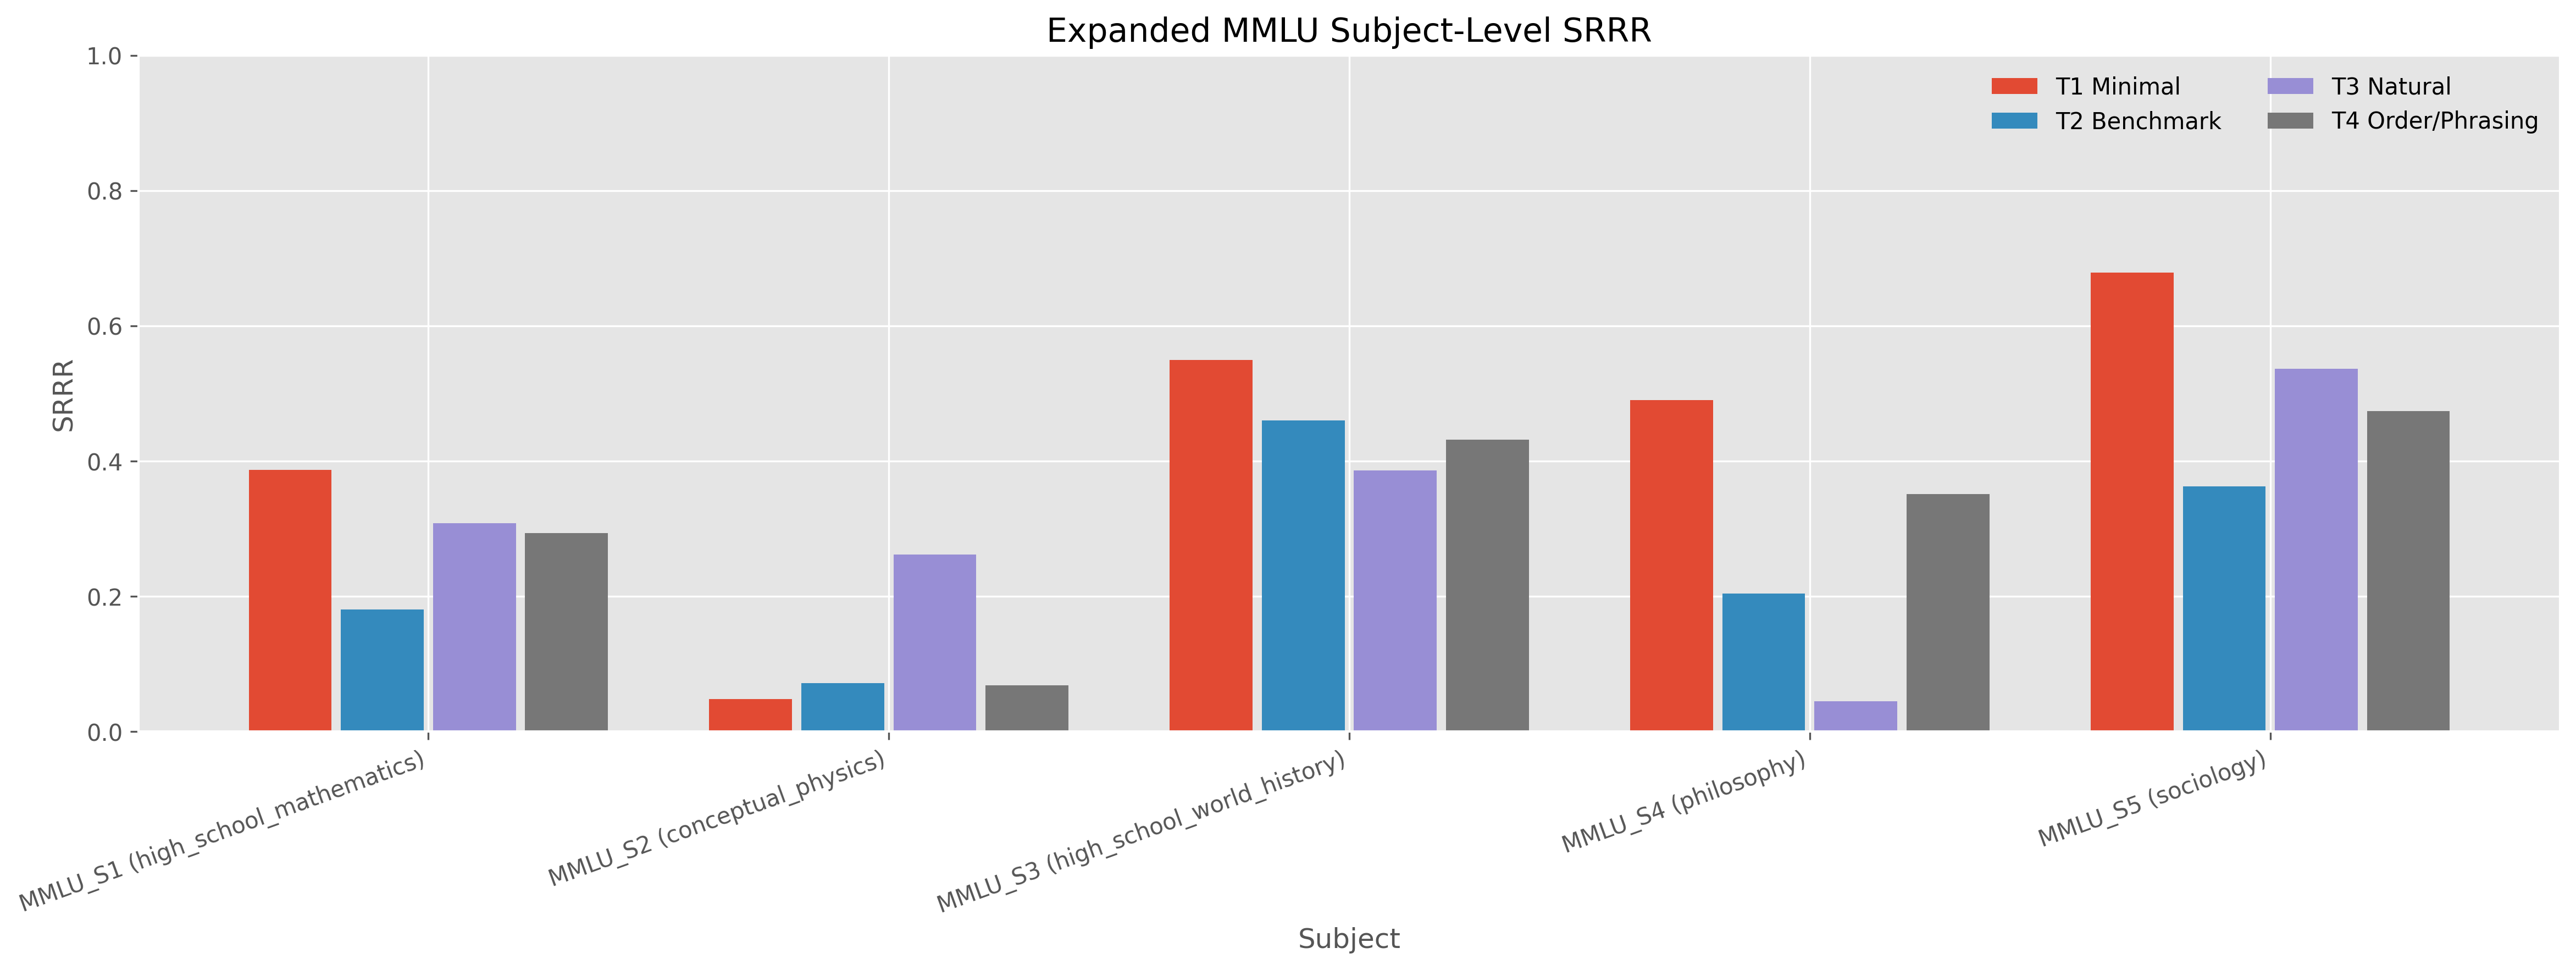
\includegraphics[width=\linewidth]{mmlu_subject_expanded_srrr.png}
\caption{Expanded MMLU subject-level SRRR. Sociology has the largest subset-induced instability under the minimal prompt.}
\label{fig:mmlu_srrr}
\end{figure}

\section{Analysis and Discussion}

\subsection{ARC-Challenge: a Robust Leaderboard Case}

ARC-Challenge behaves most like the idealized leaderboard interpretation. Gemini is first by prompt-averaged accuracy, model margins are relatively wide, and both PRRR and SRRR remain low. The maximum PRRR is 10.60\%, and the maximum SRRR is 11.20\%. This suggests that on ARC-Challenge, prompt and subset variations are usually too small to overturn the ranking.

\subsection{HellaSwag: a Fragile Leaderboard Case}

HellaSwag provides the clearest counterexample. GPT-4o-mini is first by average accuracy, but Gemini and Qwen are close enough that rank order becomes sensitive to prompt and subset choice. HellaSwag reaches a maximum PRRR of 56.00\% and a maximum SRRR of 42.80\%. This means that a single leaderboard constructed from one prompt and one subset may overstate the certainty of the top ranks.

\subsection{MMLU: Stable Aggregate Winner, Unstable Slices}

At the main dataset level, MMLU is more stable than HellaSwag but less stable than ARC-Challenge. Gemini is clearly first in the aggregate, but the middle ranks are closer. The expanded subject-level analysis shows why aggregation can hide instability: high-school world history reaches 74.30\% PRRR, and sociology reaches 67.90\% SRRR. Thus, even if the aggregate benchmark has a stable winner, subdomain-level rankings may remain fragile.

\subsection{Implications for Evaluation}

The practical implication is that leaderboard scores should be accompanied by uncertainty and rank-stability diagnostics. Average accuracy answers ``who scored highest under this setup?'' PRRR and SRRR answer a different and often more decision-relevant question: ``would the ordering survive reasonable changes to the evaluation protocol?'' For benchmark reports, especially when margins are narrow, ranking robustness should be reported rather than assumed.

\section{Limitations and Risks}

This project has several limitations. First, all evaluated tasks are multiple-choice benchmarks. The findings may not transfer directly to generation, summarization, or open-ended reasoning tasks. Second, we evaluate four models, so the observed instability patterns may differ with a larger or stronger model pool. Third, our prompt perturbations are intentionally shallow and task-preserving. This design is useful for isolating non-semantic variation, but it does not cover the full prompt design space. Fourth, our resampling protocol uses half-sized subsets without replacement; other uncertainty estimators could produce different numerical rates. Finally, API-hosted models may change over time, so exact reproducibility depends on model version stability.

\section{Conclusion}

This project asks whether LLM rankings change if we ask differently. The answer is yes, but not uniformly. ARC-Challenge remains comparatively stable, HellaSwag is strongly sensitive to prompt and subset variation, and MMLU has a stable aggregate winner but substantial subject-level instability. The main lesson is not that all leaderboards are unreliable. Rather, leaderboard reliability must be measured. A robust evaluation report should include accuracy, uncertainty, and ranking stability metrics so that users can distinguish stable superiority from narrow, protocol-dependent ordering.

\section*{Reproducibility Statement}

\begin{itemize}[leftmargin=*]
    \item Code repository: \url{https://github.com/qianchi-zhang/LLM-Ranking-Reversals}
    \item Main pipeline entrypoint: \texttt{run\_pipeline.py}
    \item Main prompt files: \texttt{data/01\_prompts.jsonl} and \texttt{data/01\_prompts\_MMLU\_subjects.jsonl}
    \item Random seeds: main data sampling seed \texttt{114514}; analysis seeds are set inside the Phase 4 scripts.
    \item Model versions: \texttt{openai/gpt-4o-mini}, \texttt{google/gemini-2.0-flash-001}, \texttt{qwen/qwen-2.5-7b-instruct}, and \texttt{meta-llama/llama-3.1-8b-instruct}.
    \item Main output directories: \texttt{data/04\_analysis/}, \texttt{data/04\_mmlu\_subject\_analysis\_expanded/}, \texttt{plots/}, and \texttt{reports/}.
\end{itemize}

\begin{thebibliography}{9}
\bibitem{clark2018arc}
Clark, P., Cowhey, I., Etzioni, O., Khot, T., Sabharwal, A., Schoenick, C., and Tafjord, O. 2018.
\textit{Think You Have Solved Question Answering? Try ARC, the AI2 Reasoning Challenge.}

\bibitem{fourrier2024openllm}
Fourrier, C., et al. 2024.
\textit{Open LLM Leaderboard v2.} Hugging Face Blog.

\bibitem{hendrycks2020mmlu}
Hendrycks, D., Burns, C., Basart, S., Zou, A., Mazeika, M., Song, D., and Steinhardt, J. 2020.
\textit{Measuring Massive Multitask Language Understanding.}

\bibitem{miller2024errorbars}
Miller, E. 2024.
\textit{Adding Error Bars to Evals: A Statistical Approach to Language Model Evaluations.}

\bibitem{zellers2019hellaswag}
Zellers, R., Holtzman, A., Bisk, Y., Farhadi, A., and Choi, Y. 2019.
\textit{HellaSwag: Can a Machine Really Finish Your Sentence?}

\bibitem{zhu2023promptrobust}
Zhu, K., Wang, J., Zhou, J., Wang, Z., Chen, H., Wang, Y., Yang, L., Ye, W., Gong, N. Z., Zhang, Y., and Xie, X. 2023.
\textit{PromptRobust: Towards Evaluating the Robustness of Large Language Models on Adversarial Prompts.}
\end{thebibliography}

\appendix

\section{Prompt Templates}

\begin{itemize}[leftmargin=*]
    \item \texttt{minimal\_instruction}: \texttt{\{question\}} + \texttt{\{choices\}} + ``Select one option.''
    \item \texttt{benchmark\_style}: ``Choose the best answer to the following multiple-choice question.'' followed by question and options.
    \item \texttt{natural\_style}: ``I have a multiple-choice question for you.'' followed by question, options, and ``Which option do you think is correct?''
    \item \texttt{order\_phrasing\_variation}: ``Consider the following question.'' followed by question, options, and ``From the four options above, select the best answer.''
\end{itemize}

\section{Additional Output Files}

\begin{itemize}[leftmargin=*]
    \item Dataset-level PRRR: \texttt{data/04\_analysis/prompt\_ranking\_reversal\_rate.csv}
    \item Dataset-level SRRR: \texttt{data/04\_analysis/subset\_ranking\_reversal\_rate.csv}
    \item Expanded MMLU subject-level PRRR: \texttt{data/04\_mmlu\_subject\_analysis\_expanded/mmlu\_subject\_prompt\_ranking\_reversal\_rate.csv}
    \item Expanded MMLU subject-level SRRR: \texttt{data/04\_mmlu\_subject\_analysis\_expanded/mmlu\_subject\_subset\_ranking\_reversal\_rate.csv}
\end{itemize}

\end{document}
